\input{Preamble.tex}

\begin{document}

%%%%%%%%%%%%%%%%%%%%%%%%%%%%%%%%%%%%%%%%%%%%%%%%%%%%%%%%%%%%%%%%%%%%%%%%% 
%								CARATULA								%
%%%%%%%%%%%%%%%%%%%%%%%%%%%%%%%%%%%%%%%%%%%%%%%%%%%%%%%%%%%%%%%%%%%%%%%%% 

\begin{titlepage}

\newcommand{\HRule}{\rule{\linewidth}{0.5mm}}
\center
\mbox{\textsc{\large \bfseries {INSTITUTO TECNOLÓGICO DE BUENOS AIRES}}}\\[1cm]
\textsc{\Large 22.42 Laboratorio de Electrónica}\\[0.5cm]


\HRule \\[0.6cm]
{ \Huge \bfseries Trabajo Práctico N$^{\circ}$4}\\[0.4cm] 
\HRule \\[1.5cm]


{\large

\emph{Grupo 3}\\
\vspace{3px}

\begin{tabular}{lr} 	
\textsc{Bertachini}, Germán  & 58750 \\ 	
\textsc{Lambertucci}, Guido Enrique  & 58009 \\
\textsc{Londero Bonaparte}, Tomás Guillermo  & 58150 \\
\textsc{Mechoulam}, Alan  &  58438\\
\textsc{Scapolla}, Franco & 58465
\end{tabular}

\vspace{20px}

\emph{Profesores}\\
\vspace{3px}
\textsc{Cossutta}, Pablo Martín\\
\textsc{Weill}, María\\
\textsc{Salvati}, Matías\\	
\vspace{100px}

\begin{tabular}{ll}

Presentado: & 15/10/19\\

\end{tabular}

}

\vfill

\end{titlepage}



%%%%%%%%%%%%%%%%%%%%%%%%%%%%%%%%%%%%%%%%%%%%%%%%%%%%%%%%%%%%%%%%%%%%%%%%% 
%								INFORME									%
%%%%%%%%%%%%%%%%%%%%%%%%%%%%%%%%%%%%%%%%%%%%%%%%%%%%%%%%%%%%%%%%%%%%%%%%%



\section{Introducción}
El circuito presentado para la medición corresponde al de una fuente conmutada como se observa en la figura ()
\begin{figure}[H]
	\centering
	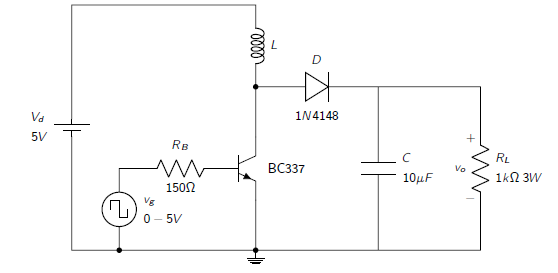
\includegraphics[width=0.9\textwidth]{Imagenes/circ.png}
\caption{Circuito fuente conmutada.}
	\label{fig:fcon}
\end{figure}

\section{Desarrollo de la experiencia}
Lo primero que se hizo fue exitar el circuito con una onda cuadrada de 0 a 5 volts, barriendo en frecuencias de 2kHz ~ 200kHz.
Se observó comparando la entrada con la salida que el circuito tiende a rectificar la señal e amplificarla, dependiendo la frecuencia amplificará mas o menos la señal, comenzando en un máximo local, que en estas condiciones coincide con el máximo absoluto, luego llegando a un mínimo local, para crecer nuevamente en el rango de frecuencias en el que se trabajó.\\
A continuación veremos algunas capturas de los puntos relevantes, siendo estos la frecuencia de inicio, la frecuencia del mínimo local, y la frecuencia final.

\begin{figure}[H]
	\centering
	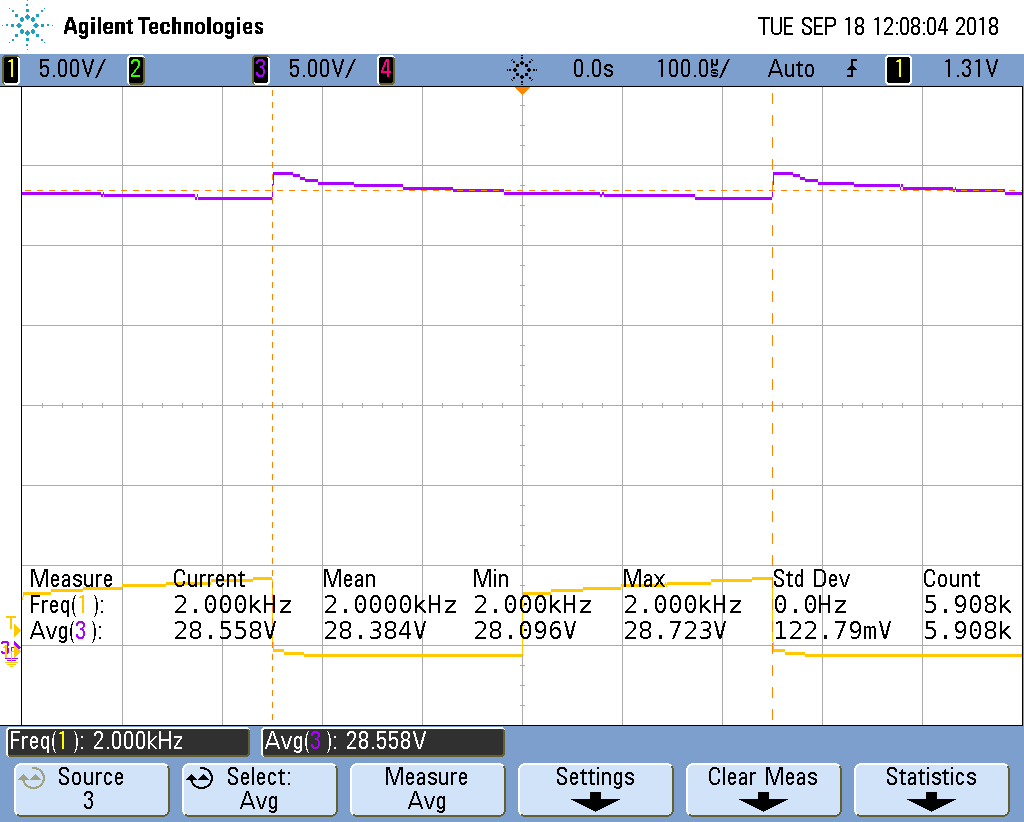
\includegraphics[width=0.9\textwidth]{Imagenes/tp3_labo3.png}
\caption{Fuente conmutada, frecuencia inicial [2kHz].}
	\label{fig:fcon}
\end{figure}

\begin{figure}[H]
	\centering
	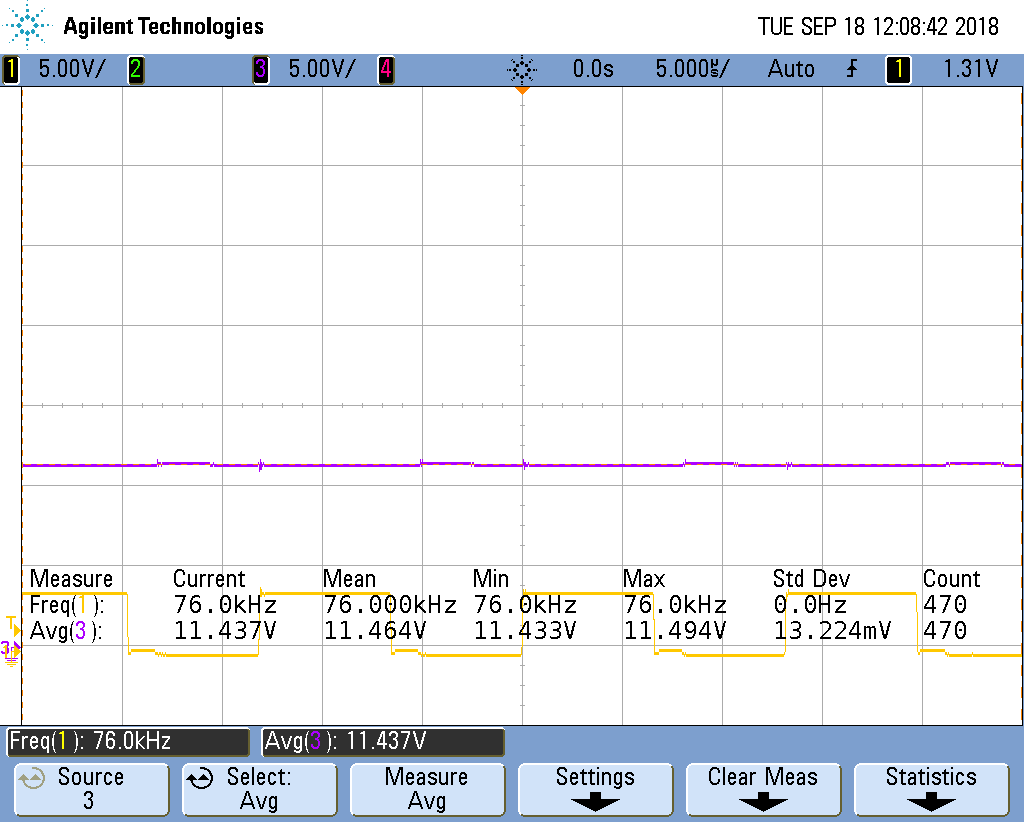
\includegraphics[width=0.9\textwidth]{Imagenes/tp3_labo4.png}
\caption{Fuente conmutada, frecuencia mínimo [76kHz].}
	\label{fig:fcon}
\end{figure}

\begin{figure}[H]
	\centering
	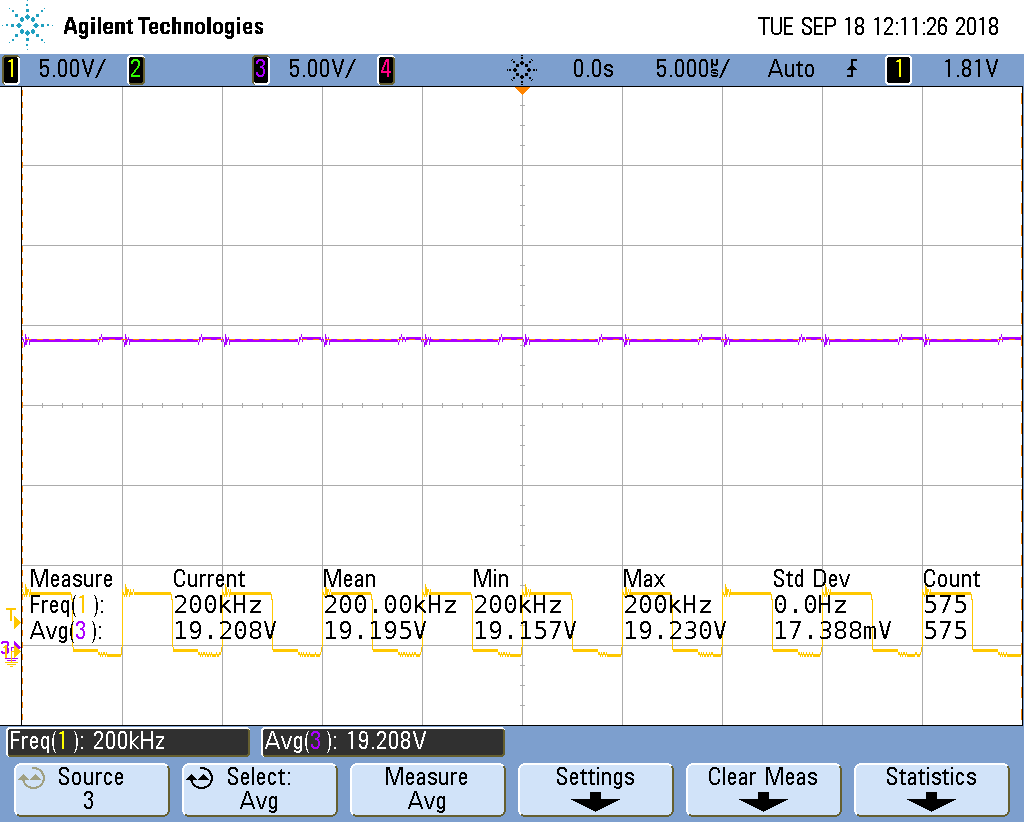
\includegraphics[width=0.9\textwidth]{Imagenes/tp3_labo5.png}
\caption{Fuente conmutada, frecuencia final [200kHz].}
	\label{fig:fcon}
\end{figure}
 
Luego, se procedió a alterar el Duty-Cycle de la señal de entrada, asi efectivamente modificando su pontencia, al aumentar el duty,  el efecto que tuvo en el circuito fue desplazar la frecuencia del mínimo hacia la continua [16kHz] al igual que agregar otro mínimo en 2kHz, un máximo local en 5kHz  la máxima tension de salida, un máximo absoluto en 100kHz  para continuar decreciendo hacia 200kHz. 
\begin{figure}[H]
	\centering
	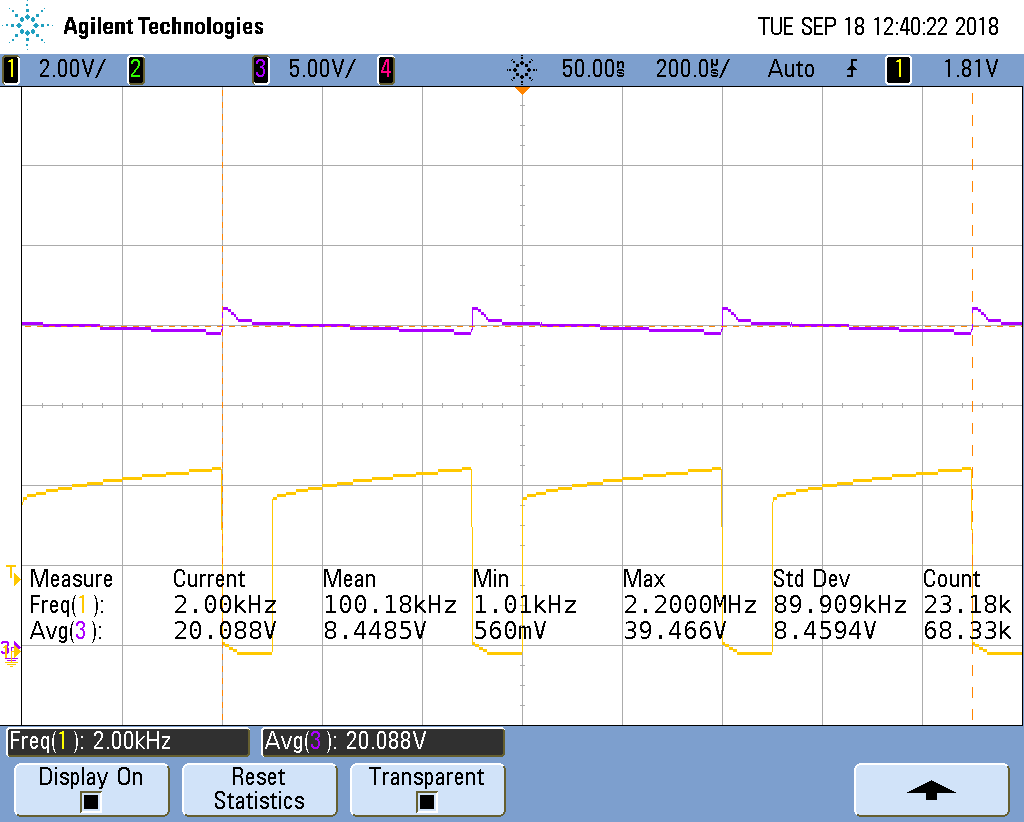
\includegraphics[width=0.9\textwidth]{Imagenes/dc_80.png}
\caption{Fuente conmutada, Duty-Cycle 80\%.}
	\label{fig:fcon}
\end{figure}
\begin{figure}[H]
	\centering
	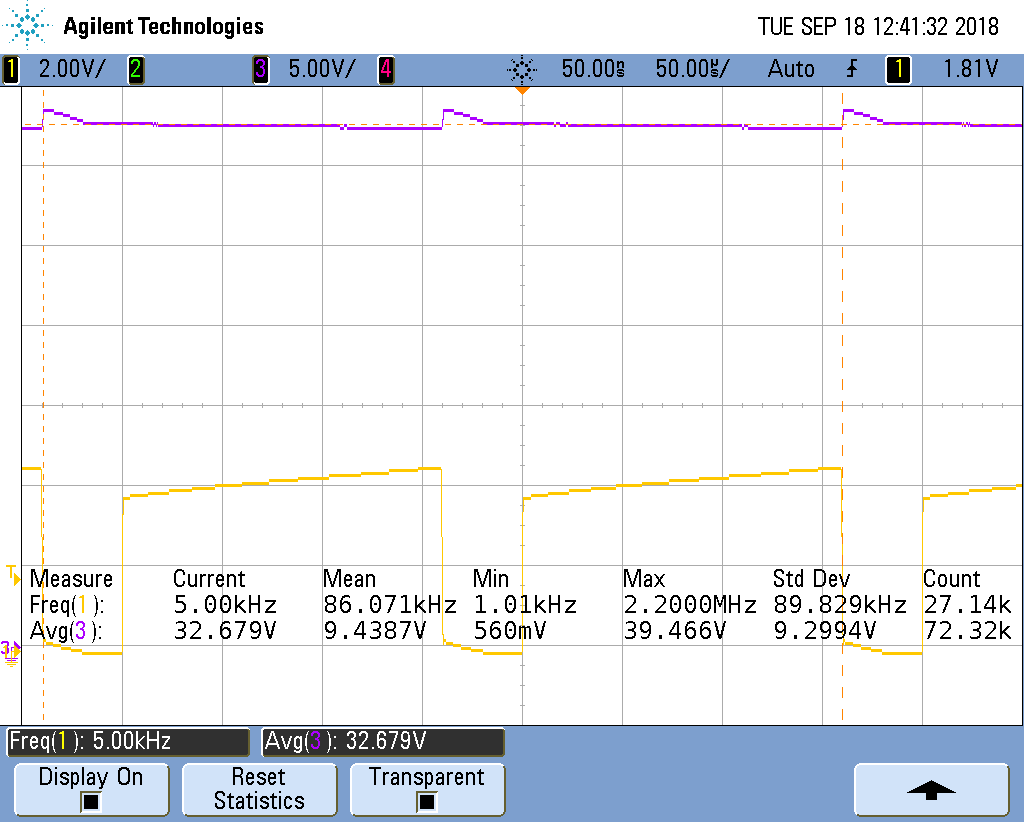
\includegraphics[width=0.9\textwidth]{Imagenes/dc_81.png}
\caption{Fuente conmutada, Duty-Cycle 80\%.}
	\label{fig:fcon}
\end{figure}
\begin{figure}[H]
	\centering
	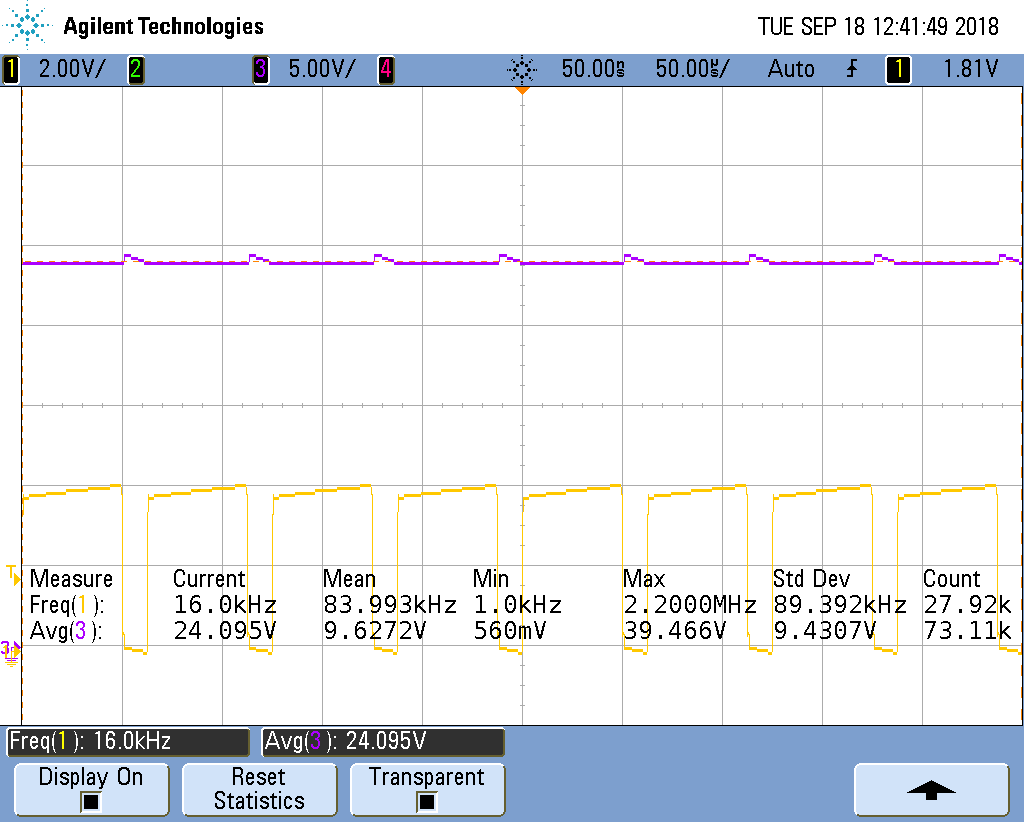
\includegraphics[width=0.9\textwidth]{Imagenes/dc_82.png}
\caption{Fuente conmutada, Duty-Cycle 80\%.}
	\label{fig:fcon}
\end{figure}
\begin{figure}[H]
	\centering
	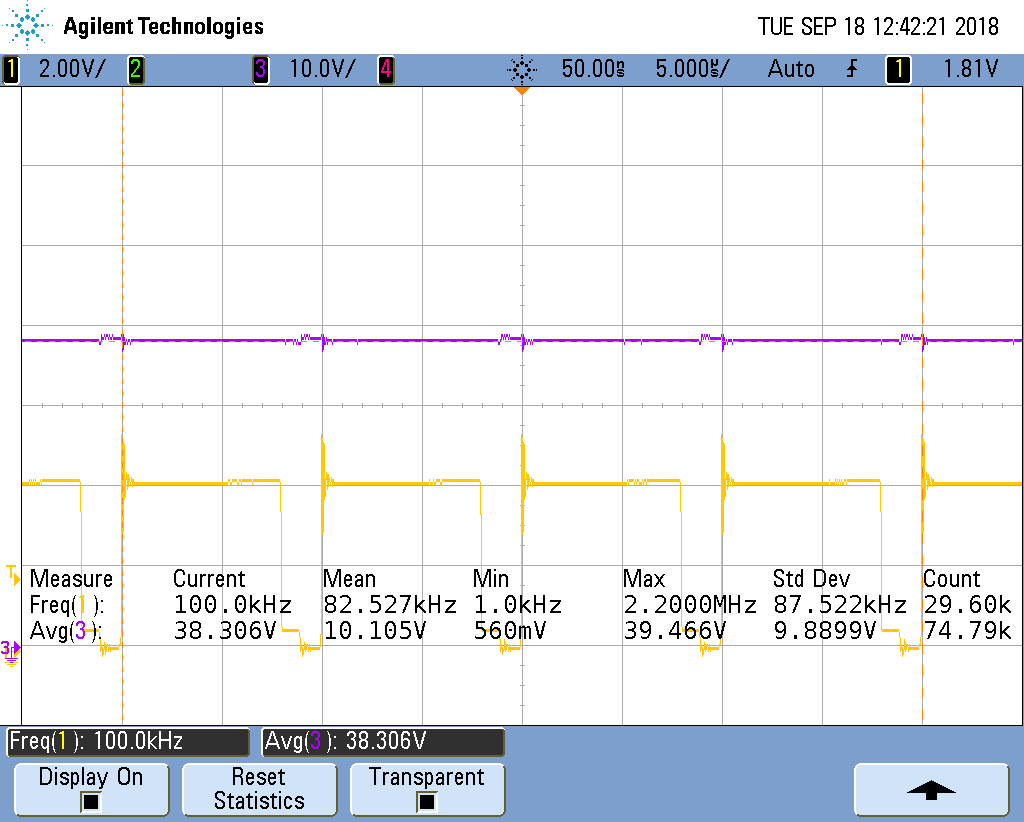
\includegraphics[width=0.9\textwidth]{Imagenes/dc_83.png}
\caption{Fuente conmutada, Duty-Cycle 80\%.}
	\label{fig:fcon}
\end{figure}
\begin{figure}[H]
	\centering
	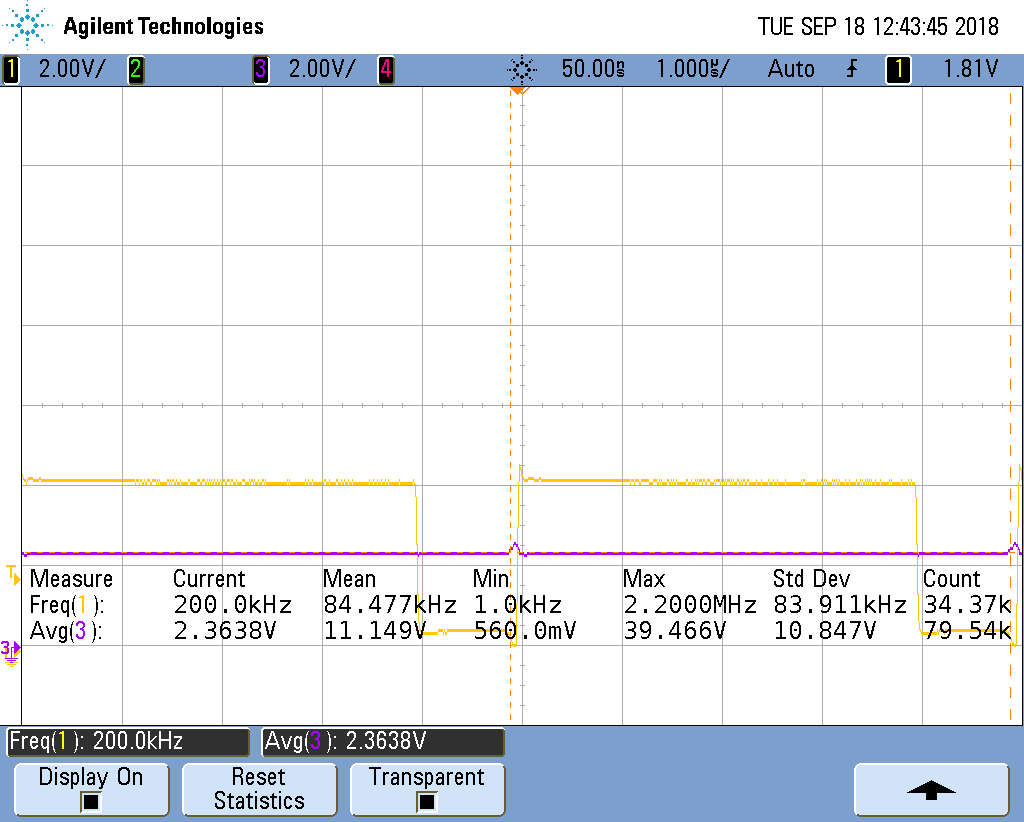
\includegraphics[width=0.9\textwidth]{Imagenes/dc_84.png}
\caption{Fuente conmutada, Duty-Cycle 80\%.}
	\label{fig:fcon}
\end{figure}
Si en cambio se baja el Duty-Cycle a 20\% comienza en un máximo local[2kHz], el cual transiciona a un mínimo local en 135kHz y finalmente se estaciona en un máximo local en 200kHz.
\begin{figure}[H]
	\centering
	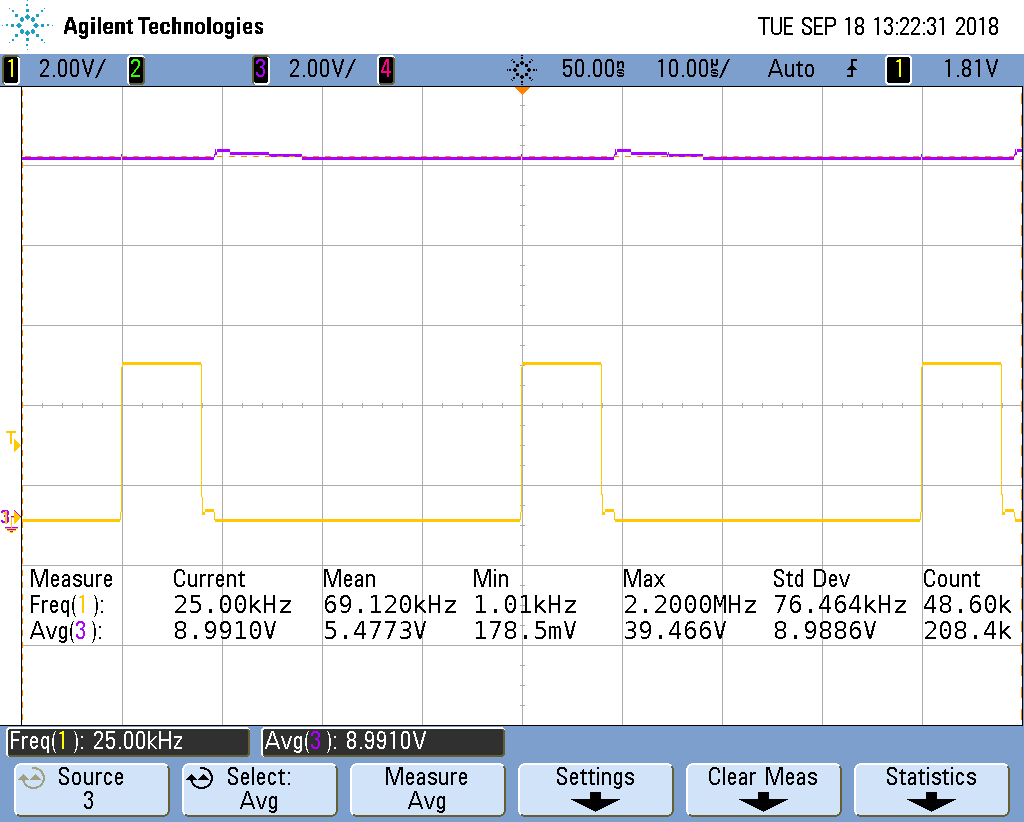
\includegraphics[width=0.9\textwidth]{Imagenes/dc_20.png}
\caption{Fuente conmutada, Duty-Cycle 20\%.}
	\label{fig:fcon}
\end{figure}
\begin{figure}[H]
	\centering
	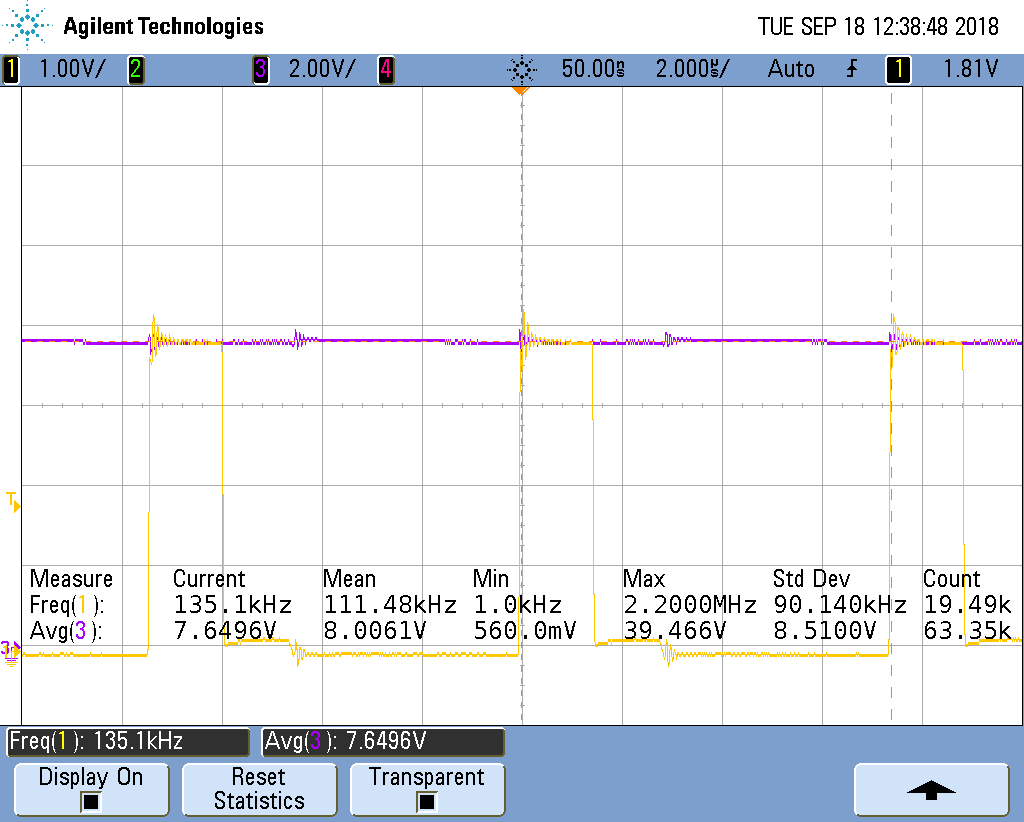
\includegraphics[width=0.9\textwidth]{Imagenes/dc_21.png}
\caption{Fuente conmutada, Duty-Cycle 20\%.}
	\label{fig:fcon}
\end{figure}
\begin{figure}[H]
	\centering
	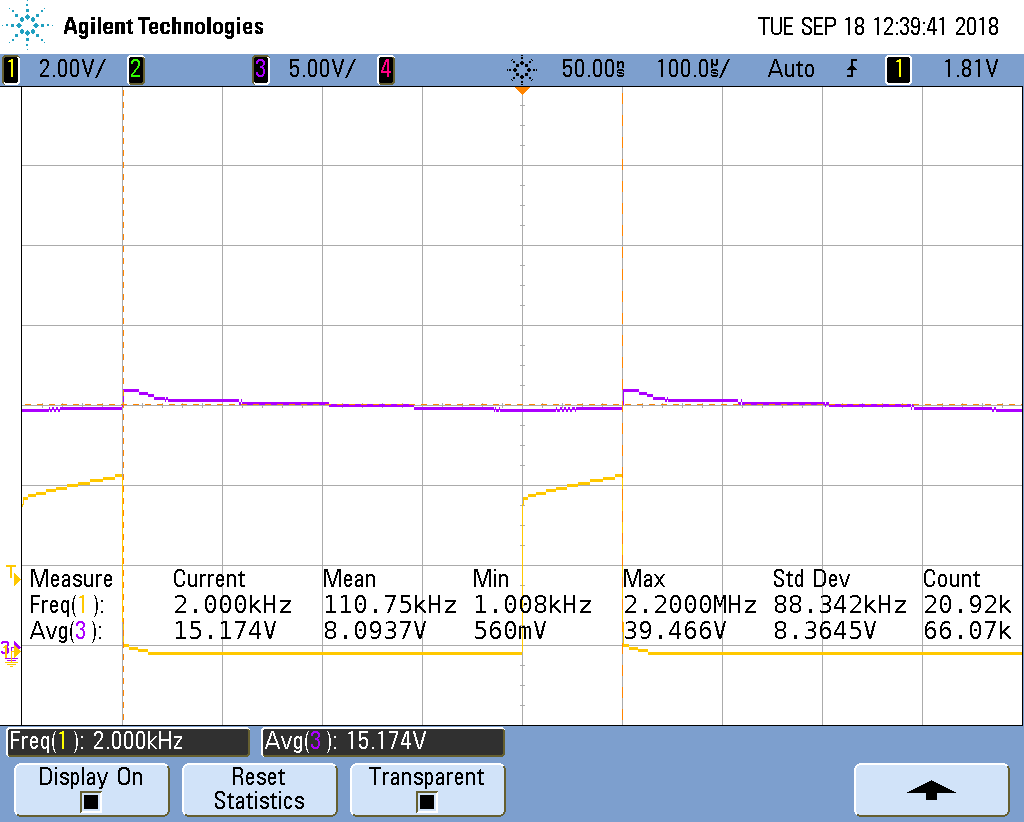
\includegraphics[width=0.9\textwidth]{Imagenes/dc_22.png}
\caption{Fuente conmutada, Duty-Cycle 20\%.}
	\label{fig:fcon}
\end{figure}

Se continuó por medir la respuesta al escalon del circuito en condiciones nominales obtenienod el siguiente gráfico:
\begin{figure}[H]
	\centering
	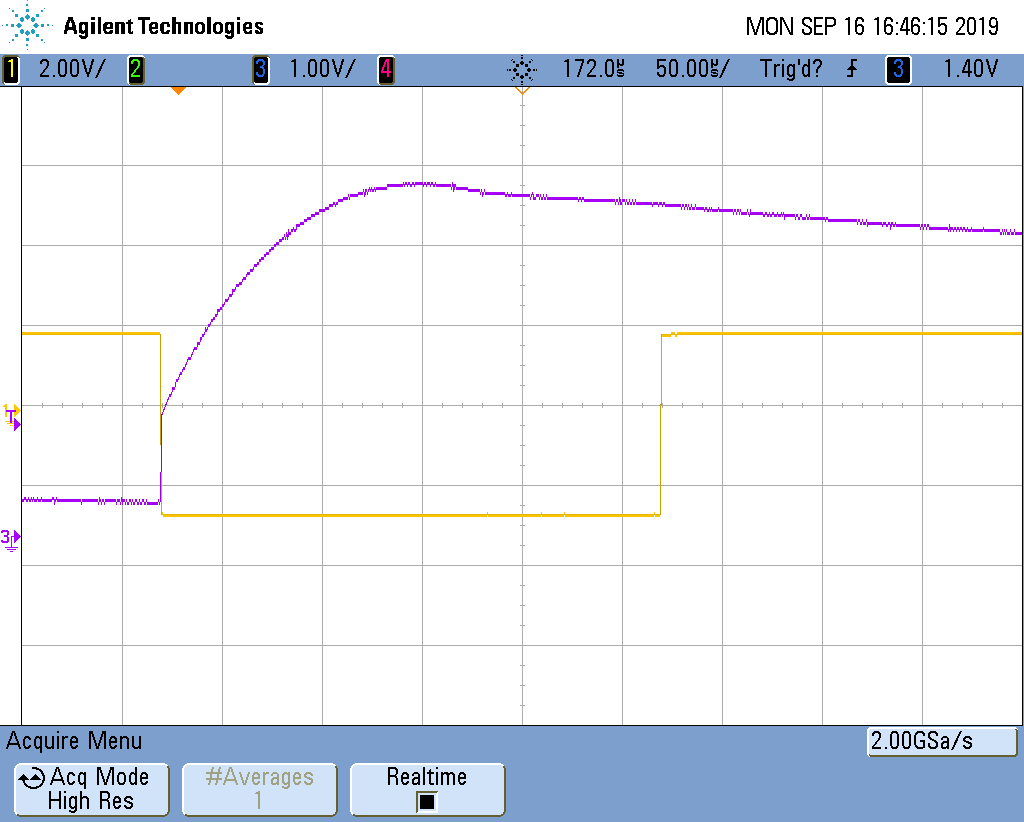
\includegraphics[width=0.9\textwidth]{Imagenes/tp3_labo7.png}
\caption{Fuente conmutada, frecuencia final [200kHz].}
	\label{fig:fcon}
\end{figure}

\end{document}
